\section{Deep Convolutional Neural Network}
\label{sec:cnn}

This chapter serves as an introduction to the basic notions that will come up in the remaining of this thesis, namely the notion of \gls{nn} and \gls{cnn}.
We start by introducing generalities about gls{nn}.
Most of the content of the present chapter is taken from \cite{goodfellow16}.

\subsection{Neural Network}
Deep learning essentially refers to a family of machine learning methods that historically derive from the \gls{mlp}, also known as Neural Network.
An \gls{mlp} aims at approximating a function $f^{*}$ with a function $f(x;\theta)$ parameterized by $\theta$.
More concretely, an \gls{mlp} converts an input $x$ to an output $y$ using a chain of function $f^{(1)} \circ f^{2} \circ \cdots \circ f^{n}(x)$, which justifies its name ``network''.
Each function is usually referred to as ``layer'', while the term ``neural'' comes from the fact that it is originally inspired by neuroscience \cite{mcculloch43}.

As in all machine learning setup, one wants to find the set of parameters $\bm{\theta}$ so as to optimize a cost function, for example the \gls{mse}:

\begin{equation}
\mathcal{L}(\bm{theta}) = \sum_{x\in \mathcal{X}}(f^{*}(x)-f(x;\bm{\theta}))
\end{equation}

One typically use a gradient-descent method to solve the above problem.

In the frame of \gls{mlp}, the functions $f^{m}(x;\bm{\theta_{m}})$ are linear (or fully-connected) layer, i.e. $\bm{theta}_m=(\bm{w)}_{m},b$, followed by an activation function $\sigma(.)$

\begin{equation}
f^{m}(x;\bm{\theta_{m}}) = \sigma(\bm{x}^{T}\bm{w} + b)
\end{equation}

The activation function, allows to inject non-linearities in the model.
Such function is applied element-wise.
The \gls{relu} is the most widespread.
It writes:

\begin{equation}
\sigma(x) = \max \{0, \bm{x}\}
\end{equation}

\subsection{Convolutional Network}
Many machine learning applications relie on structured data, i.e. data that respect a grid-like topology.
Typical examples include time-series and images.
For this reason, \cite{lecun95} introduced the notion of convolutional network, which adapts the previous MLP to leverage the grid-like topolgy in an effective manner.
In particular, the author replaces one or several layers of an MLP with convolutional layers.
In the case of (discrete) images, the convolution operator writes:

\begin{equation}
S(i,j) = (I * K)(i,j) = \sum_{m} \sum_{n} I(m,n) K(i-m, j-n)
\end{equation}

where $I$ is a grayscale image and $K$ is a kernel.
This formulation naturally extends to multi-channel images.
The convolutional operator brings the following advantage over the \gls{mlp}: (1) It naturally leverages the spatial connectivity of pixels.
(2) As the size of the kernel is usually much smaller than the input size (sparse-connectivity), the number of parameters are greatly reduced, which reduces the memory consumption, accelerates the training and improves performances \cite{lecun95}.
Fig. \ref{fig:cnn_con} illustrates the idea of sparse connectivity brought by convolutional layers.

\begin{figure}[!htpb]
  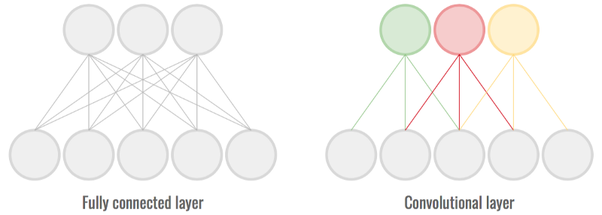
\includegraphics[width=13cm]{theory/fc_vs_conv}
  \caption{(Left) A fully-connected (linear) layer with 1D input at the bottom. (Right) Convolutional layer with a kernel of size 3.}
  \label{fig:cnn_con}
\end{figure}

\subsubsection{Pooling}

Another important component of Convolutional networks are pooling layers, which allow to increase the receptive field of the convolutional operators as the depth is increased.
This effectively allow to capture, in the case of images, visual features at different spatial scales, i.e. that gets more global as the depth increases.
In particular, the max-pooling operator computes for each spatial location the maximal filter response over a pre-defined neighborhood (see fig. \ref{fig:max_pool})

\begin{figure}[!htpb]
  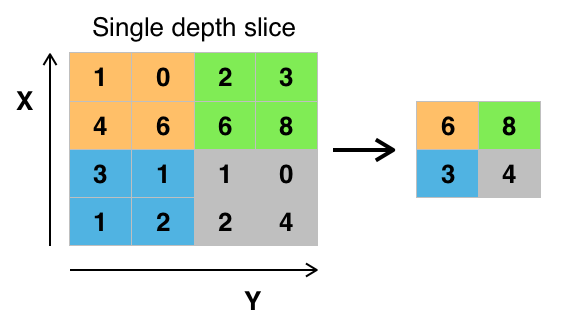
\includegraphics[width=13cm]{theory/max_pooling}
  \caption{(Left) Input. (Right) Output of max-pooling layer. Each color represents a set of values included in the sliding window.}
  \label{fig:max_pool}
\end{figure}
Figure \ref{fig:cnn} illustrates a CNN applied to an image processing task.

\subsubsection{Optimization}
Since the advent of deep learning, many optimization algorithms have been proposed and proved to be effective, each with their own pros and cons.
To name a few: \gls{sgd}, Adam \cite{kingma14}, and RMSProp \cite{tieleman12}.
As the two latter are essentially improvements of \gls{sgd}, we restrict this section to \gls{sgd} (see \ref{alg:sgd}).
In practice, effectively training a deep learning model demands careful study of hyper-parameters.
The most crucial is certainly the learning rate $\lambda$ which controls the fraction of gradient-estimate one wants to use to update $\bm{\theta}$.
Also, one needs to initialize $\bm{\theta}$ to random values.
The latter step has been an important object of study, e.g \cite{he15}, \cite{glorot10}.

\begin{algorithm}[H]
  \label{alg:sgd}
 \caption{Stochastic Gradient Descent (SGD)}

 \begin{algorithmic}[1]
  \Require{Training data ${(\bm{x}_{i},y_{j})}_{i=1}^{N}$, learning rate $\lambda$, initial parameters $\bm{\theta}$}
  \Ensure{Model parameters $\bm{\theta}$}
  \Repeat
    \State Sample a minibatch of m examples from the training set $\{(\bm{x}_{1},y_{1}), \cdots, (\bm{x}_{m},y_{m})\}$
    \State Compute gradient estimate: $\hat{\bm{g}} \leftarrow + \frac{1}{m} \nabla_{\bm{\theta}}\sum_{i}\mathcal{L}(f(\bm{x}_{i}; \bm{\theta}), y_{i})$
    \State Apply gradient update: $\bm{\theta} \leftarrow \bm{\theta} - \lambda \hat{\bm{g}}$
    \Until {stopping criterion is met}
  \end{algorithmic}
\end{algorithm}


\subsubsection{Batch normalization}
As already mentioned, training a CNN demands a careful tuning of the learning rate in order to converge to a proper solution.
Practical issues such as exploding/vanishing gradient arise when the latter is two high/low, respectively.
In particular, as noted in \cite{ioffe15}, the input distribution of a given layer is dependent on the parameters of all preceding layers, a phenomenon called internal covariate shift.
To circumvent the latter problem, a batch normalization can be added at the output of each layer to normalize the values of a given minibatch to a normal distribution.
Additionally, such normalization often needs to combine with an activation function, and therefore will have its left tail zeroed-out in the case of a \gls{relu}.
To circumvent that, authors add learnable scaling and shifting parameters, $\gamma$ and $\beta$, respectively.
Also, batch normalization also has a regularization effect due to fluctuations in mini-batch statistics \cite{gastaldi17}.
The algorithm is described in alg. \ref{alg:batchnorm}.

\begin{algorithm}[H]
  \label{alg:batchnorm}
 \caption{Batch Normalization}
 \begin{algorithmic}[1]
  \Require{Minibatch of size $M$: $\mathcal{B}=\{(\bm{x}_{i})\}_{i=1}^{M}$, learnable scaling and shifting parameters, $\gamma$ and $\beta$}
  \Ensure{$\bm{x}'_{i}=\text{BN}(\bm{x}_{i};\gamma,\beta)$}
    \State Compute mean: $\mu_{\mathcal{B}}\leftarrow \frac{1}{m}\sum_{i=1}^{M}\bm{x}_{i}$

    \State Compute variance: $\sigma^{2}_{\mathcal{B}}\leftarrow \frac{1}{m}\sum_{i=1}^{M}(\bm{x}_{i}-\mu_{\mathcal{B}})$

    \State Normalize: $\hat{\bm{x}}_{i}\leftarrow \frac{\bm{x}_{i}-\mu_{\mathcal{B}}}{\sqrt{\sigma^{2}_{\mathcal{B}} + \epsilon}}$

    \State Scale and shift: $x_{i}'\leftarrow \gamma \hat{\bm{x}}_{i} + \beta \equiv \text{BN}(\bm{x}_{i};\gamma,\beta)$

 \end{algorithmic}
\end{algorithm}

\begin{figure}[!htpb]
  \centering
  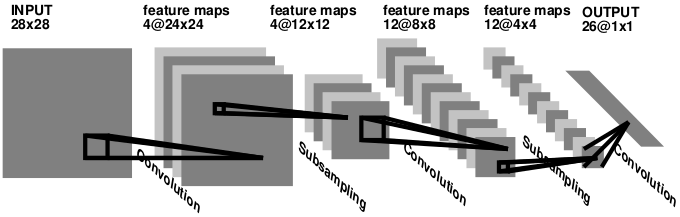
\includegraphics[width=13cm]{theory/cnn}
  \caption{Convolutional Neural Network applied to an image task.
    The network applies a succession of convolution, and pooling (subsampling) operation.
  Activation functions are not represented. Figure taken from \cite{lecun95}}
  \label{fig:cnn}
\end{figure}

\subsection{Convolutional Autoencoder}
The basic idea of \gls{ae}, first introduced in \cite{vincent10}, consists in training a model in an unsupervised manner, so as to generate a compressed representation of the input.
Such compressed representation, often called feature vector, is typically used in a subsequent machine learning task.
In particular, an \gls{ae} is composed of two modules: An encoding function $f_{\theta}$, and a decoding function $g_{\phi}$.
The training objective is to minimize the discrepancy between an input sample $x$ and its reconstructed version $x'$.
An example is shown on Fig. \ref{fig:ae}.

For example, using the \gls{mse} criterion, one writes:

\begin{equation}
\mathcal{L}_{AE} = \mathbb{E}_{x_{i}}||f_{\theta}(g_{\phi}(x)) - x ||
\end{equation}


\begin{figure}[!htpb]
  \centering
  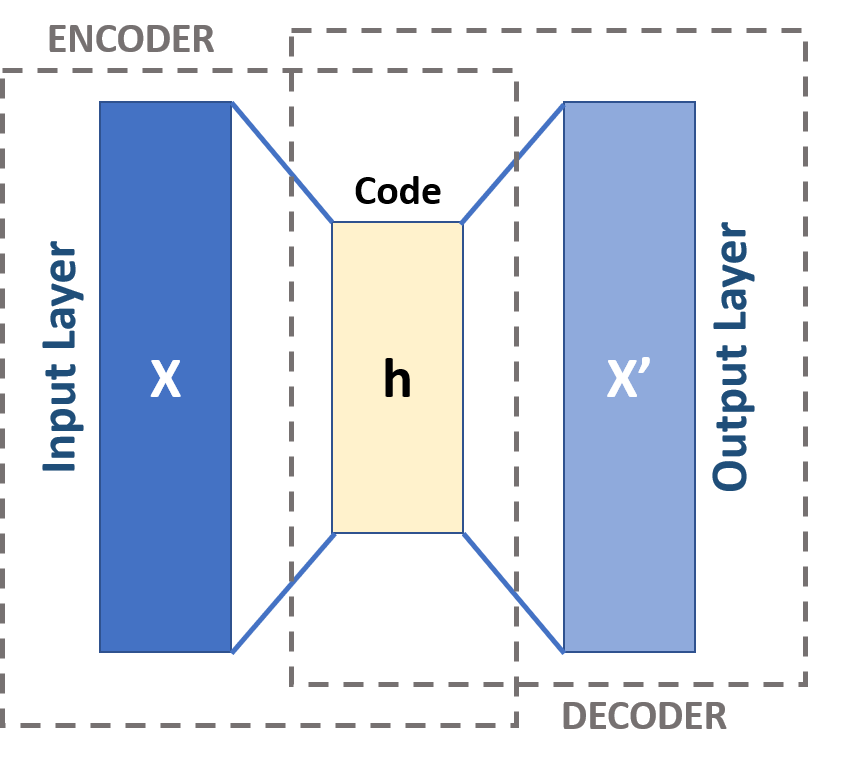
\includegraphics[width=7cm]{theory/ae}
  \caption{Convolutional Autoencoder.
    The input sample $x$ passes through an encoder.
    The output of the encoder, called $h$, passes through a decoder to give the reconstructed version $x'$.
    In yellow is the bottleneck.}
  \label{fig:ae}
\end{figure}


%%% Local Variables:
%%% mode: latex
%%% TeX-master: "../../main"
%%% End:
